\documentclass[1p]{elsarticle_modified}
%\bibliographystyle{elsarticle-num}

%\usepackage[colorlinks]{hyperref}
%\usepackage{abbrmath_seonhwa} %\Abb, \Ascr, \Acal ,\Abf, \Afrak
\usepackage{amsfonts}
\usepackage{amssymb}
\usepackage{amsmath}
\usepackage{amsthm}
\usepackage{scalefnt}
\usepackage{amsbsy}
\usepackage{kotex}
\usepackage{caption}
\usepackage{subfig}
\usepackage{color}
\usepackage{graphicx}
\usepackage{xcolor} %% white, black, red, green, blue, cyan, magenta, yellow
\usepackage{float}
\usepackage{setspace}
\usepackage{hyperref}

\usepackage{tikz}
\usetikzlibrary{arrows}

\usepackage{multirow}
\usepackage{array} % fixed length table
\usepackage{hhline}

%%%%%%%%%%%%%%%%%%%%%
\makeatletter
\renewcommand*\env@matrix[1][\arraystretch]{%
	\edef\arraystretch{#1}%
	\hskip -\arraycolsep
	\let\@ifnextchar\new@ifnextchar
	\array{*\c@MaxMatrixCols c}}
\makeatother %https://tex.stackexchange.com/questions/14071/how-can-i-increase-the-line-spacing-in-a-matrix
%%%%%%%%%%%%%%%

\usepackage[normalem]{ulem}

\newcommand{\msout}[1]{\ifmmode\text{\sout{\ensuremath{#1}}}\else\sout{#1}\fi}
%SOURCE: \msout is \stkout macro in https://tex.stackexchange.com/questions/20609/strikeout-in-math-mode

\newcommand{\cancel}[1]{
	\ifmmode
	{\color{red}\msout{#1}}
	\else
	{\color{red}\sout{#1}}
	\fi
}

\newcommand{\add}[1]{
	{\color{blue}\uwave{#1}}
}

\newcommand{\replace}[2]{
	\ifmmode
	{\color{red}\msout{#1}}{\color{blue}\uwave{#2}}
	\else
	{\color{red}\sout{#1}}{\color{blue}\uwave{#2}}
	\fi
}

\newcommand{\Sol}{\mathcal{S}} %segment
\newcommand{\D}{D} %diagram
\newcommand{\A}{\mathcal{A}} %arc


%%%%%%%%%%%%%%%%%%%%%%%%%%%%%5 test

\def\sl{\operatorname{\textup{SL}}(2,\Cbb)}
\def\psl{\operatorname{\textup{PSL}}(2,\Cbb)}
\def\quan{\mkern 1mu \triangleright \mkern 1mu}

\theoremstyle{definition}
\newtheorem{thm}{Theorem}[section]
\newtheorem{prop}[thm]{Proposition}
\newtheorem{lem}[thm]{Lemma}
\newtheorem{ques}[thm]{Question}
\newtheorem{cor}[thm]{Corollary}
\newtheorem{defn}[thm]{Definition}
\newtheorem{exam}[thm]{Example}
\newtheorem{rmk}[thm]{Remark}
\newtheorem{alg}[thm]{Algorithm}

\newcommand{\I}{\sqrt{-1}}
\begin{document}

%\begin{frontmatter}
%
%\title{Boundary parabolic representations of knots up to 8 crossings}
%
%%% Group authors per affiliation:
%\author{Yunhi Cho} 
%\address{Department of Mathematics, University of Seoul, Seoul, Korea}
%\ead{yhcho@uos.ac.kr}
%
%
%\author{Seonhwa Kim} %\fnref{s_kim}}
%\address{Center for Geometry and Physics, Institute for Basic Science, Pohang, 37673, Korea}
%\ead{ryeona17@ibs.re.kr}
%
%\author{Hyuk Kim}
%\address{Department of Mathematical Sciences, Seoul National University, Seoul 08826, Korea}
%\ead{hyukkim@snu.ac.kr}
%
%\author{Seokbeom Yoon}
%\address{Department of Mathematical Sciences, Seoul National University, Seoul, 08826,  Korea}
%\ead{sbyoon15@snu.ac.kr}
%
%\begin{abstract}
%We find all boundary parabolic representation of knots up to 8 crossings.
%
%\end{abstract}
%\begin{keyword}
%    \MSC[2010] 57M25 
%\end{keyword}
%
%\end{frontmatter}

%\linenumbers
%\tableofcontents
%
\newcommand\colored[1]{\textcolor{white}{\rule[-0.35ex]{0.8em}{1.4ex}}\kern-0.8em\color{red} #1}%
%\newcommand\colored[1]{\textcolor{white}{ #1}\kern-2.17ex	\textcolor{white}{ #1}\kern-1.81ex	\textcolor{white}{ #1}\kern-2.15ex\color{red}#1	}

{\Large $\underline{12a_{0057}~(K12a_{0057})}$}

\setlength{\tabcolsep}{10pt}
\renewcommand{\arraystretch}{1.6}
\vspace{1cm}\begin{tabular}{m{100pt}>{\centering\arraybackslash}m{274pt}}
\multirow{5}{120pt}{
	\centering
	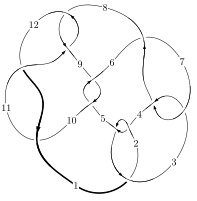
\includegraphics[width=112pt]{../../../GIT/diagram.site/Diagrams/png/858_12a_0057.png}\\
\ \ \ A knot diagram\footnotemark}&
\allowdisplaybreaks
\textbf{Linearized knot diagam} \\
\cline{2-2}
 &
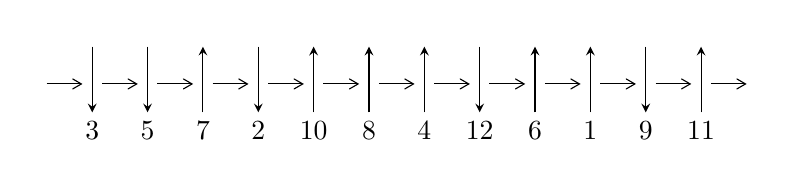
\begin{tikzpicture}[x=20pt, y=17pt]
	% nodes
	\node (C0) at (0, 0) {};
	\node (C1) at (1, 0) {};
	\node (C1U) at (1, +1) {};
	\node (C1D) at (1, -1) {3};

	\node (C2) at (2, 0) {};
	\node (C2U) at (2, +1) {};
	\node (C2D) at (2, -1) {5};

	\node (C3) at (3, 0) {};
	\node (C3U) at (3, +1) {};
	\node (C3D) at (3, -1) {7};

	\node (C4) at (4, 0) {};
	\node (C4U) at (4, +1) {};
	\node (C4D) at (4, -1) {2};

	\node (C5) at (5, 0) {};
	\node (C5U) at (5, +1) {};
	\node (C5D) at (5, -1) {10};

	\node (C6) at (6, 0) {};
	\node (C6U) at (6, +1) {};
	\node (C6D) at (6, -1) {8};

	\node (C7) at (7, 0) {};
	\node (C7U) at (7, +1) {};
	\node (C7D) at (7, -1) {4};

	\node (C8) at (8, 0) {};
	\node (C8U) at (8, +1) {};
	\node (C8D) at (8, -1) {12};

	\node (C9) at (9, 0) {};
	\node (C9U) at (9, +1) {};
	\node (C9D) at (9, -1) {6};

	\node (C10) at (10, 0) {};
	\node (C10U) at (10, +1) {};
	\node (C10D) at (10, -1) {1};

	\node (C11) at (11, 0) {};
	\node (C11U) at (11, +1) {};
	\node (C11D) at (11, -1) {9};

	\node (C12) at (12, 0) {};
	\node (C12U) at (12, +1) {};
	\node (C12D) at (12, -1) {11};
	\node (C13) at (13, 0) {};

	% arrows
	\draw[->,>={angle 60}]
	(C0) edge (C1) (C1) edge (C2) (C2) edge (C3) (C3) edge (C4) (C4) edge (C5) (C5) edge (C6) (C6) edge (C7) (C7) edge (C8) (C8) edge (C9) (C9) edge (C10) (C10) edge (C11) (C11) edge (C12) (C12) edge (C13) ;	\draw[->,>=stealth]
	(C1U) edge (C1D) (C2U) edge (C2D) (C3D) edge (C3U) (C4U) edge (C4D) (C5D) edge (C5U) (C6D) edge (C6U) (C7D) edge (C7U) (C8U) edge (C8D) (C9D) edge (C9U) (C10D) edge (C10U) (C11U) edge (C11D) (C12D) edge (C12U) ;
	\end{tikzpicture} \\
\hhline{~~} \\& 
\textbf{Solving Sequence} \\ \cline{2-2} 
 &
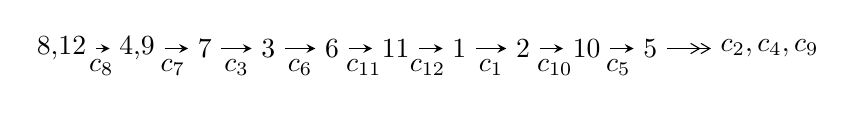
\begin{tikzpicture}[x=23pt, y=7pt]
	% node
	\node (A0) at (-1/8, 0) {8,12};
	\node (A1) at (17/16, 0) {4,9};
	\node (A2) at (17/8, 0) {7};
	\node (A3) at (25/8, 0) {3};
	\node (A4) at (33/8, 0) {6};
	\node (A5) at (41/8, 0) {11};
	\node (A6) at (49/8, 0) {1};
	\node (A7) at (57/8, 0) {2};
	\node (A8) at (65/8, 0) {10};
	\node (A9) at (73/8, 0) {5};
	\node (C1) at (1/2, -1) {$c_{8}$};
	\node (C2) at (13/8, -1) {$c_{7}$};
	\node (C3) at (21/8, -1) {$c_{3}$};
	\node (C4) at (29/8, -1) {$c_{6}$};
	\node (C5) at (37/8, -1) {$c_{11}$};
	\node (C6) at (45/8, -1) {$c_{12}$};
	\node (C7) at (53/8, -1) {$c_{1}$};
	\node (C8) at (61/8, -1) {$c_{10}$};
	\node (C9) at (69/8, -1) {$c_{5}$};
	\node (A10) at (11, 0) {$c_{2},c_{4},c_{9}$};

	% edge
	\draw[->,>=stealth]	
	(A0) edge (A1) (A1) edge (A2) (A2) edge (A3) (A3) edge (A4) (A4) edge (A5) (A5) edge (A6) (A6) edge (A7) (A7) edge (A8) (A8) edge (A9) ;
	\draw[->>,>={angle 60}]	
	(A9) edge (A10);
\end{tikzpicture} \\ 

\end{tabular} \\

\footnotetext{
The image of knot diagram is generated by the software ``\textbf{Draw programme}" developed by Andrew Bartholomew(\url{http://www.layer8.co.uk/maths/draw/index.htm\#Running-draw}), where we modified some parts for our purpose(\url{https://github.com/CATsTAILs/LinksPainter}).
}\phantom \\ \newline 
\centering \textbf{Ideals for irreducible components\footnotemark of $X_{\text{par}}$} 
 
\begin{align*}
I^u_{1}&=\langle 
6.97582\times10^{34} u^{103}+6.61069\times10^{35} u^{102}+\cdots+1.52431\times10^{34} b+1.69169\times10^{35},\\
\phantom{I^u_{1}}&\phantom{= \langle  }1.01712\times10^{35} u^{103}+8.18175\times10^{35} u^{102}+\cdots+2.17758\times10^{33} a+1.06317\times10^{35},\;u^{104}+8 u^{103}+\cdots+26 u^2+1\rangle \\
I^u_{2}&=\langle 
3 a^5 u+9 a^5-19 a^4 u+8 a^4-32 a^3 u+47 a^3-27 a^2 u-16 a^2-64 a u+13 b+29 a-15 u+7,\\
\phantom{I^u_{2}}&\phantom{= \langle  }a^6- a^5 u-4 a^4 u+5 a^4- a^3 u- a^3-7 a^2 u+3 a^2-3 a u+2 a- u+1,\;u^2- u+1\rangle \\
I^u_{3}&=\langle 
b,\;- u^3-2 u^2+a-2 u,\;u^4+u^3+u^2+1\rangle \\
\\
\end{align*}
\raggedright * 3 irreducible components of $\dim_{\mathbb{C}}=0$, with total 120 representations.\\
\footnotetext{All coefficients of polynomials are rational numbers. But the coefficients are sometimes approximated in decimal forms when there is not enough margin.}
\newpage
\renewcommand{\arraystretch}{1}
\centering \section*{I. $I^u_{1}= \langle 6.98\times10^{34} u^{103}+6.61\times10^{35} u^{102}+\cdots+1.52\times10^{34} b+1.69\times10^{35},\;1.02\times10^{35} u^{103}+8.18\times10^{35} u^{102}+\cdots+2.18\times10^{33} a+1.06\times10^{35},\;u^{104}+8 u^{103}+\cdots+26 u^2+1 \rangle$}
\flushleft \textbf{(i) Arc colorings}\\
\begin{tabular}{m{7pt} m{180pt} m{7pt} m{180pt} }
\flushright $a_{8}=$&$\begin{pmatrix}1\\0\end{pmatrix}$ \\
\flushright $a_{12}=$&$\begin{pmatrix}0\\u\end{pmatrix}$ \\
\flushright $a_{4}=$&$\begin{pmatrix}-46.7086 u^{103}-375.726 u^{102}+\cdots+7.43615 u-48.8233\\-4.57639 u^{103}-43.3685 u^{102}+\cdots+5.03677 u-11.0981\end{pmatrix}$ \\
\flushright $a_{9}=$&$\begin{pmatrix}1\\u^2\end{pmatrix}$ \\
\flushright $a_{7}=$&$\begin{pmatrix}6.85333 u^{103}+66.2746 u^{102}+\cdots-8.70012 u+9.69003\\-3.32389 u^{103}-36.2817 u^{102}+\cdots+12.7191 u-9.19042\end{pmatrix}$ \\
\flushright $a_{3}=$&$\begin{pmatrix}-97.9649 u^{103}-736.860 u^{102}+\cdots-12.7281 u-70.4352\\-47.5278 u^{103}-414.116 u^{102}+\cdots+50.0294 u-79.6418\end{pmatrix}$ \\
\flushright $a_{6}=$&$\begin{pmatrix}10.1772 u^{103}+102.556 u^{102}+\cdots-21.4192 u+18.8804\\-3.32389 u^{103}-36.2817 u^{102}+\cdots+12.7191 u-9.19042\end{pmatrix}$ \\
\flushright $a_{11}=$&$\begin{pmatrix}u\\u^3+u\end{pmatrix}$ \\
\flushright $a_{1}=$&$\begin{pmatrix}u^3\\u^5+u^3+u\end{pmatrix}$ \\
\flushright $a_{2}=$&$\begin{pmatrix}36.4714 u^{103}+295.722 u^{102}+\cdots-1.60920 u+35.1731\\5.67709 u^{103}+42.1133 u^{102}+\cdots+5.76655 u+5.64315\end{pmatrix}$ \\
\flushright $a_{10}=$&$\begin{pmatrix}u^5+u\\u^7+u^5+2 u^3+u\end{pmatrix}$ \\
\flushright $a_{5}=$&$\begin{pmatrix}-38.2688 u^{103}-287.431 u^{102}+\cdots+5.82490 u-35.2283\\-16.9340 u^{103}-158.639 u^{102}+\cdots+30.8364 u-34.3757\end{pmatrix}$\\&\end{tabular}
\flushleft \textbf{(ii) Obstruction class $= -1$}\\~\\
\flushleft \textbf{(iii) Cusp Shapes $= 68.6439 u^{103}+557.865 u^{102}+\cdots-39.8300 u+80.6891$}\\~\\
\newpage\renewcommand{\arraystretch}{1}
\flushleft \textbf{(iv) u-Polynomials at the component}\newline \\
\begin{tabular}{m{50pt}|m{274pt}}
Crossings & \hspace{64pt}u-Polynomials at each crossing \\
\hline $$\begin{aligned}c_{1}\end{aligned}$$&$\begin{aligned}
&u^{104}+57 u^{103}+\cdots-38 u+1
\end{aligned}$\\
\hline $$\begin{aligned}c_{2},c_{4}\end{aligned}$$&$\begin{aligned}
&u^{104}-7 u^{103}+\cdots-2 u+1
\end{aligned}$\\
\hline $$\begin{aligned}c_{3},c_{7}\end{aligned}$$&$\begin{aligned}
&u^{104}-3 u^{103}+\cdots+56 u+16
\end{aligned}$\\
\hline $$\begin{aligned}c_{5},c_{9}\end{aligned}$$&$\begin{aligned}
&u^{104}+2 u^{103}+\cdots+8192 u+4096
\end{aligned}$\\
\hline $$\begin{aligned}c_{6}\end{aligned}$$&$\begin{aligned}
&u^{104}-33 u^{103}+\cdots-3136 u+256
\end{aligned}$\\
\hline $$\begin{aligned}c_{8},c_{11}\end{aligned}$$&$\begin{aligned}
&u^{104}-8 u^{103}+\cdots+26 u^2+1
\end{aligned}$\\
\hline $$\begin{aligned}c_{10},c_{12}\end{aligned}$$&$\begin{aligned}
&u^{104}-32 u^{103}+\cdots-52 u+1
\end{aligned}$\\
\hline
\end{tabular}\\~\\
\newpage\renewcommand{\arraystretch}{1}
\flushleft \textbf{(v) Riley Polynomials at the component}\newline \\
\begin{tabular}{m{50pt}|m{274pt}}
Crossings & \hspace{64pt}Riley Polynomials at each crossing \\
\hline $$\begin{aligned}c_{1}\end{aligned}$$&$\begin{aligned}
&y^{104}-13 y^{103}+\cdots+1086 y+1
\end{aligned}$\\
\hline $$\begin{aligned}c_{2},c_{4}\end{aligned}$$&$\begin{aligned}
&y^{104}-57 y^{103}+\cdots+38 y+1
\end{aligned}$\\
\hline $$\begin{aligned}c_{3},c_{7}\end{aligned}$$&$\begin{aligned}
&y^{104}-33 y^{103}+\cdots-3136 y+256
\end{aligned}$\\
\hline $$\begin{aligned}c_{5},c_{9}\end{aligned}$$&$\begin{aligned}
&y^{104}+70 y^{103}+\cdots+251658240 y+16777216
\end{aligned}$\\
\hline $$\begin{aligned}c_{6}\end{aligned}$$&$\begin{aligned}
&y^{104}+71 y^{103}+\cdots+4435968 y+65536
\end{aligned}$\\
\hline $$\begin{aligned}c_{8},c_{11}\end{aligned}$$&$\begin{aligned}
&y^{104}+32 y^{103}+\cdots+52 y+1
\end{aligned}$\\
\hline $$\begin{aligned}c_{10},c_{12}\end{aligned}$$&$\begin{aligned}
&y^{104}+88 y^{103}+\cdots+772 y+1
\end{aligned}$\\
\hline
\end{tabular}\\~\\
\newpage\flushleft \textbf{(vi) Complex Volumes and Cusp Shapes}
$$\begin{array}{c|c|c}  
\text{Solutions to }I^u_{1}& \I (\text{vol} + \sqrt{-1}CS) & \text{Cusp shape}\\
 \hline 
\begin{aligned}
u &= \phantom{-}0.020101 + 0.968920 I \\
a &= -1.62773 + 0.60872 I \\
b &= \phantom{-}1.104780 + 0.011234 I\end{aligned}
 & \phantom{-}4.85259 - 0.00883 I & \phantom{-0.000000 } 0 \\ \hline\begin{aligned}
u &= \phantom{-}0.020101 - 0.968920 I \\
a &= -1.62773 - 0.60872 I \\
b &= \phantom{-}1.104780 - 0.011234 I\end{aligned}
 & \phantom{-}4.85259 + 0.00883 I & \phantom{-0.000000 } 0 \\ \hline\begin{aligned}
u &= \phantom{-}0.088929 + 1.032320 I \\
a &= \phantom{-}1.54140 - 0.10414 I \\
b &= -1.106510 + 0.209872 I\end{aligned}
 & \phantom{-}4.42375 - 4.85437 I & \phantom{-0.000000 } 0 \\ \hline\begin{aligned}
u &= \phantom{-}0.088929 - 1.032320 I \\
a &= \phantom{-}1.54140 + 0.10414 I \\
b &= -1.106510 - 0.209872 I\end{aligned}
 & \phantom{-}4.42375 + 4.85437 I & \phantom{-0.000000 } 0 \\ \hline\begin{aligned}
u &= \phantom{-}0.508673 + 0.806106 I \\
a &= -1.67780 - 3.42402 I \\
b &= \phantom{-}0.259513 - 0.337681 I\end{aligned}
 & -1.76705 - 1.65580 I & \phantom{-0.000000 } 0 \\ \hline\begin{aligned}
u &= \phantom{-}0.508673 - 0.806106 I \\
a &= -1.67780 + 3.42402 I \\
b &= \phantom{-}0.259513 + 0.337681 I\end{aligned}
 & -1.76705 + 1.65580 I & \phantom{-0.000000 } 0 \\ \hline\begin{aligned}
u &= -0.724250 + 0.757923 I \\
a &= -0.249685 + 0.014515 I \\
b &= -1.214800 + 0.436033 I\end{aligned}
 & -1.03612 - 4.58038 I & \phantom{-0.000000 } 0 \\ \hline\begin{aligned}
u &= -0.724250 - 0.757923 I \\
a &= -0.249685 - 0.014515 I \\
b &= -1.214800 - 0.436033 I\end{aligned}
 & -1.03612 + 4.58038 I & \phantom{-0.000000 } 0 \\ \hline\begin{aligned}
u &= \phantom{-}0.551150 + 0.900436 I \\
a &= \phantom{-}0.76590 + 2.14805 I \\
b &= \phantom{-}0.163285 + 0.546485 I\end{aligned}
 & -1.41743 - 2.62965 I & \phantom{-0.000000 } 0 \\ \hline\begin{aligned}
u &= \phantom{-}0.551150 - 0.900436 I \\
a &= \phantom{-}0.76590 - 2.14805 I \\
b &= \phantom{-}0.163285 - 0.546485 I\end{aligned}
 & -1.41743 + 2.62965 I & \phantom{-0.000000 } 0\\
 \hline 
 \end{array}$$\newpage$$\begin{array}{c|c|c}  
\text{Solutions to }I^u_{1}& \I (\text{vol} + \sqrt{-1}CS) & \text{Cusp shape}\\
 \hline 
\begin{aligned}
u &= \phantom{-}0.700965 + 0.624043 I \\
a &= \phantom{-}0.821618 + 0.490951 I \\
b &= \phantom{-}0.853960 + 0.159820 I\end{aligned}
 & \phantom{-}0.063961 + 0.318270 I & \phantom{-0.000000 } 0 \\ \hline\begin{aligned}
u &= \phantom{-}0.700965 - 0.624043 I \\
a &= \phantom{-}0.821618 - 0.490951 I \\
b &= \phantom{-}0.853960 - 0.159820 I\end{aligned}
 & \phantom{-}0.063961 - 0.318270 I & \phantom{-0.000000 } 0 \\ \hline\begin{aligned}
u &= -0.711021 + 0.819449 I \\
a &= -0.086162 + 0.367371 I \\
b &= \phantom{-}1.233520 - 0.260497 I\end{aligned}
 & \phantom{-}0.360291 + 0.869699 I & \phantom{-0.000000 } 0 \\ \hline\begin{aligned}
u &= -0.711021 - 0.819449 I \\
a &= -0.086162 - 0.367371 I \\
b &= \phantom{-}1.233520 + 0.260497 I\end{aligned}
 & \phantom{-}0.360291 - 0.869699 I & \phantom{-0.000000 } 0 \\ \hline\begin{aligned}
u &= \phantom{-}0.338448 + 0.821183 I \\
a &= \phantom{-}0.439609 - 0.068020 I \\
b &= -0.203409 - 0.340268 I\end{aligned}
 & \phantom{-}0.32890 - 1.53001 I & \phantom{-0.000000 } 0 \\ \hline\begin{aligned}
u &= \phantom{-}0.338448 - 0.821183 I \\
a &= \phantom{-}0.439609 + 0.068020 I \\
b &= -0.203409 + 0.340268 I\end{aligned}
 & \phantom{-}0.32890 + 1.53001 I & \phantom{-0.000000 } 0 \\ \hline\begin{aligned}
u &= \phantom{-}0.371975 + 1.056300 I \\
a &= \phantom{-}0.219181 + 0.313047 I \\
b &= -0.737120 - 0.575993 I\end{aligned}
 & \phantom{-}0.284397 - 1.151140 I & \phantom{-0.000000 } 0 \\ \hline\begin{aligned}
u &= \phantom{-}0.371975 - 1.056300 I \\
a &= \phantom{-}0.219181 - 0.313047 I \\
b &= -0.737120 + 0.575993 I\end{aligned}
 & \phantom{-}0.284397 + 1.151140 I & \phantom{-0.000000 } 0 \\ \hline\begin{aligned}
u &= \phantom{-}0.763473 + 0.833575 I \\
a &= \phantom{-}1.23213 + 1.16646 I \\
b &= \phantom{-}0.825340 + 0.691127 I\end{aligned}
 & -2.19732 - 0.20425 I & \phantom{-0.000000 } 0 \\ \hline\begin{aligned}
u &= \phantom{-}0.763473 - 0.833575 I \\
a &= \phantom{-}1.23213 - 1.16646 I \\
b &= \phantom{-}0.825340 - 0.691127 I\end{aligned}
 & -2.19732 + 0.20425 I & \phantom{-0.000000 } 0\\
 \hline 
 \end{array}$$\newpage$$\begin{array}{c|c|c}  
\text{Solutions to }I^u_{1}& \I (\text{vol} + \sqrt{-1}CS) & \text{Cusp shape}\\
 \hline 
\begin{aligned}
u &= \phantom{-}0.307670 + 1.089840 I \\
a &= -1.52467 - 1.13055 I \\
b &= \phantom{-}0.781449 - 0.708430 I\end{aligned}
 & -3.12443 - 2.29817 I & \phantom{-0.000000 } 0 \\ \hline\begin{aligned}
u &= \phantom{-}0.307670 - 1.089840 I \\
a &= -1.52467 + 1.13055 I \\
b &= \phantom{-}0.781449 + 0.708430 I\end{aligned}
 & -3.12443 + 2.29817 I & \phantom{-0.000000 } 0 \\ \hline\begin{aligned}
u &= \phantom{-}0.277505 + 1.104830 I \\
a &= -0.1271100 - 0.0362554 I \\
b &= \phantom{-}0.688170 + 0.874892 I\end{aligned}
 & -2.91862 - 4.97555 I & \phantom{-0.000000 } 0 \\ \hline\begin{aligned}
u &= \phantom{-}0.277505 - 1.104830 I \\
a &= -0.1271100 + 0.0362554 I \\
b &= \phantom{-}0.688170 - 0.874892 I\end{aligned}
 & -2.91862 + 4.97555 I & \phantom{-0.000000 } 0 \\ \hline\begin{aligned}
u &= -0.760110 + 0.849074 I \\
a &= \phantom{-}0.534218 - 1.195980 I \\
b &= -0.182890 - 1.029530 I\end{aligned}
 & -4.67900 + 0.62095 I & \phantom{-0.000000 } 0 \\ \hline\begin{aligned}
u &= -0.760110 - 0.849074 I \\
a &= \phantom{-}0.534218 + 1.195980 I \\
b &= -0.182890 + 1.029530 I\end{aligned}
 & -4.67900 - 0.62095 I & \phantom{-0.000000 } 0 \\ \hline\begin{aligned}
u &= \phantom{-}0.239231 + 1.116540 I \\
a &= \phantom{-}1.36880 + 0.80283 I \\
b &= -0.978221 + 0.642817 I\end{aligned}
 & \phantom{-}1.11393 - 6.06429 I & \phantom{-0.000000 } 0 \\ \hline\begin{aligned}
u &= \phantom{-}0.239231 - 1.116540 I \\
a &= \phantom{-}1.36880 - 0.80283 I \\
b &= -0.978221 - 0.642817 I\end{aligned}
 & \phantom{-}1.11393 + 6.06429 I & \phantom{-0.000000 } 0 \\ \hline\begin{aligned}
u &= -0.888885 + 0.718904 I \\
a &= -0.531734 + 1.184580 I \\
b &= -1.048580 + 0.760099 I\end{aligned}
 & -6.53896 - 5.97441 I & \phantom{-0.000000 } 0 \\ \hline\begin{aligned}
u &= -0.888885 - 0.718904 I \\
a &= -0.531734 - 1.184580 I \\
b &= -1.048580 - 0.760099 I\end{aligned}
 & -6.53896 + 5.97441 I & \phantom{-0.000000 } 0\\
 \hline 
 \end{array}$$\newpage$$\begin{array}{c|c|c}  
\text{Solutions to }I^u_{1}& \I (\text{vol} + \sqrt{-1}CS) & \text{Cusp shape}\\
 \hline 
\begin{aligned}
u &= \phantom{-}0.849313 + 0.087081 I \\
a &= \phantom{-}0.56368 - 1.29841 I \\
b &= \phantom{-}0.969631 - 0.765873 I\end{aligned}
 & -6.10338 - 7.37044 I & \phantom{-0.000000 } 0 \\ \hline\begin{aligned}
u &= \phantom{-}0.849313 - 0.087081 I \\
a &= \phantom{-}0.56368 + 1.29841 I \\
b &= \phantom{-}0.969631 + 0.765873 I\end{aligned}
 & -6.10338 + 7.37044 I & \phantom{-0.000000 } 0 \\ \hline\begin{aligned}
u &= \phantom{-}0.146678 + 0.835966 I \\
a &= \phantom{-}0.508790 + 0.043311 I \\
b &= \phantom{-}0.025150 - 0.703991 I\end{aligned}
 & \phantom{-}0.50382 - 1.71842 I & \phantom{-0.000000 } 0 \\ \hline\begin{aligned}
u &= \phantom{-}0.146678 - 0.835966 I \\
a &= \phantom{-}0.508790 - 0.043311 I \\
b &= \phantom{-}0.025150 + 0.703991 I\end{aligned}
 & \phantom{-}0.50382 + 1.71842 I & \phantom{-0.000000 } 0 \\ \hline\begin{aligned}
u &= -0.914130 + 0.710133 I \\
a &= \phantom{-}0.66641 - 1.29667 I \\
b &= \phantom{-}1.065570 - 0.825694 I\end{aligned}
 & -9.8021 - 11.2187 I & \phantom{-0.000000 } 0 \\ \hline\begin{aligned}
u &= -0.914130 - 0.710133 I \\
a &= \phantom{-}0.66641 + 1.29667 I \\
b &= \phantom{-}1.065570 + 0.825694 I\end{aligned}
 & -9.8021 + 11.2187 I & \phantom{-0.000000 } 0 \\ \hline\begin{aligned}
u &= \phantom{-}0.765930 + 0.869765 I \\
a &= -0.02115 + 2.55065 I \\
b &= -0.791634 + 0.793650 I\end{aligned}
 & -5.87770 - 1.49881 I & \phantom{-0.000000 } 0 \\ \hline\begin{aligned}
u &= \phantom{-}0.765930 - 0.869765 I \\
a &= -0.02115 - 2.55065 I \\
b &= -0.791634 - 0.793650 I\end{aligned}
 & -5.87770 + 1.49881 I & \phantom{-0.000000 } 0 \\ \hline\begin{aligned}
u &= -0.892156 + 0.739909 I \\
a &= \phantom{-}0.30564 + 1.68316 I \\
b &= \phantom{-}0.759500 + 0.991887 I\end{aligned}
 & -10.79950 - 4.57831 I & \phantom{-0.000000 } 0 \\ \hline\begin{aligned}
u &= -0.892156 - 0.739909 I \\
a &= \phantom{-}0.30564 - 1.68316 I \\
b &= \phantom{-}0.759500 - 0.991887 I\end{aligned}
 & -10.79950 + 4.57831 I & \phantom{-0.000000 } 0\\
 \hline 
 \end{array}$$\newpage$$\begin{array}{c|c|c}  
\text{Solutions to }I^u_{1}& \I (\text{vol} + \sqrt{-1}CS) & \text{Cusp shape}\\
 \hline 
\begin{aligned}
u &= \phantom{-}0.549237 + 1.021450 I \\
a &= \phantom{-}0.277415 + 1.180080 I \\
b &= -0.913257 - 0.043795 I\end{aligned}
 & \phantom{-}1.67910 - 1.36015 I & \phantom{-0.000000 } 0 \\ \hline\begin{aligned}
u &= \phantom{-}0.549237 - 1.021450 I \\
a &= \phantom{-}0.277415 - 1.180080 I \\
b &= -0.913257 + 0.043795 I\end{aligned}
 & \phantom{-}1.67910 + 1.36015 I & \phantom{-0.000000 } 0 \\ \hline\begin{aligned}
u &= -0.704293 + 0.925402 I \\
a &= -0.520684 + 1.249690 I \\
b &= \phantom{-}1.256970 + 0.183413 I\end{aligned}
 & \phantom{-}0.69382 + 4.56111 I & \phantom{-0.000000 } 0 \\ \hline\begin{aligned}
u &= -0.704293 - 0.925402 I \\
a &= -0.520684 - 1.249690 I \\
b &= \phantom{-}1.256970 - 0.183413 I\end{aligned}
 & \phantom{-}0.69382 - 4.56111 I & \phantom{-0.000000 } 0 \\ \hline\begin{aligned}
u &= -0.888784 + 0.755463 I \\
a &= \phantom{-}0.292839 - 1.319880 I \\
b &= \phantom{-}0.949109 - 0.740773 I\end{aligned}
 & -11.11310 - 1.60376 I & \phantom{-0.000000 } 0 \\ \hline\begin{aligned}
u &= -0.888784 - 0.755463 I \\
a &= \phantom{-}0.292839 + 1.319880 I \\
b &= \phantom{-}0.949109 + 0.740773 I\end{aligned}
 & -11.11310 + 1.60376 I & \phantom{-0.000000 } 0 \\ \hline\begin{aligned}
u &= \phantom{-}0.812047 + 0.837491 I \\
a &= -1.39732 - 1.12186 I \\
b &= -0.953304 - 0.748451 I\end{aligned}
 & -5.37858 + 4.30990 I & \phantom{-0.000000 } 0 \\ \hline\begin{aligned}
u &= \phantom{-}0.812047 - 0.837491 I \\
a &= -1.39732 + 1.12186 I \\
b &= -0.953304 + 0.748451 I\end{aligned}
 & -5.37858 - 4.30990 I & \phantom{-0.000000 } 0 \\ \hline\begin{aligned}
u &= -0.872599 + 0.774567 I \\
a &= -0.21957 - 1.49195 I \\
b &= -0.674295 - 0.904933 I\end{aligned}
 & -7.68839 + 0.16391 I & \phantom{-0.000000 } 0 \\ \hline\begin{aligned}
u &= -0.872599 - 0.774567 I \\
a &= -0.21957 + 1.49195 I \\
b &= -0.674295 + 0.904933 I\end{aligned}
 & -7.68839 - 0.16391 I & \phantom{-0.000000 } 0\\
 \hline 
 \end{array}$$\newpage$$\begin{array}{c|c|c}  
\text{Solutions to }I^u_{1}& \I (\text{vol} + \sqrt{-1}CS) & \text{Cusp shape}\\
 \hline 
\begin{aligned}
u &= -0.768255 + 0.881229 I \\
a &= \phantom{-}1.090040 - 0.500963 I \\
b &= -0.955497 + 0.043580 I\end{aligned}
 & -6.17949 + 2.90009 I & \phantom{-0.000000 } 0 \\ \hline\begin{aligned}
u &= -0.768255 - 0.881229 I \\
a &= \phantom{-}1.090040 + 0.500963 I \\
b &= -0.955497 - 0.043580 I\end{aligned}
 & -6.17949 - 2.90009 I & \phantom{-0.000000 } 0 \\ \hline\begin{aligned}
u &= \phantom{-}0.761656 + 0.891292 I \\
a &= -1.30304 - 1.35327 I \\
b &= -0.757619 - 0.846783 I\end{aligned}
 & -5.81140 - 4.27423 I & \phantom{-0.000000 } 0 \\ \hline\begin{aligned}
u &= \phantom{-}0.761656 - 0.891292 I \\
a &= -1.30304 + 1.35327 I \\
b &= -0.757619 + 0.846783 I\end{aligned}
 & -5.81140 + 4.27423 I & \phantom{-0.000000 } 0 \\ \hline\begin{aligned}
u &= -0.125362 + 0.816549 I \\
a &= -1.60573 + 1.61861 I \\
b &= \phantom{-}1.037850 + 0.456374 I\end{aligned}
 & \phantom{-}3.10305 + 2.04932 I & \phantom{-0.000000 } 0 \\ \hline\begin{aligned}
u &= -0.125362 - 0.816549 I \\
a &= -1.60573 - 1.61861 I \\
b &= \phantom{-}1.037850 - 0.456374 I\end{aligned}
 & \phantom{-}3.10305 - 2.04932 I & \phantom{-0.000000 } 0 \\ \hline\begin{aligned}
u &= -0.209971 + 0.797600 I \\
a &= \phantom{-}1.38225 - 1.86157 I \\
b &= -1.090740 - 0.631167 I\end{aligned}
 & \phantom{-}0.79834 + 7.03577 I & \phantom{-0.000000 } 0 \\ \hline\begin{aligned}
u &= -0.209971 - 0.797600 I \\
a &= \phantom{-}1.38225 + 1.86157 I \\
b &= -1.090740 + 0.631167 I\end{aligned}
 & \phantom{-}0.79834 - 7.03577 I & \phantom{-0.000000 } 0 \\ \hline\begin{aligned}
u &= -0.751265 + 0.907966 I \\
a &= -0.782532 + 0.938819 I \\
b &= -0.104033 + 1.028450 I\end{aligned}
 & -4.49816 + 5.10320 I & \phantom{-0.000000 } 0 \\ \hline\begin{aligned}
u &= -0.751265 - 0.907966 I \\
a &= -0.782532 - 0.938819 I \\
b &= -0.104033 - 1.028450 I\end{aligned}
 & -4.49816 - 5.10320 I & \phantom{-0.000000 } 0\\
 \hline 
 \end{array}$$\newpage$$\begin{array}{c|c|c}  
\text{Solutions to }I^u_{1}& \I (\text{vol} + \sqrt{-1}CS) & \text{Cusp shape}\\
 \hline 
\begin{aligned}
u &= \phantom{-}0.629659 + 0.996600 I \\
a &= -0.15233 - 1.68044 I \\
b &= \phantom{-}0.966172 - 0.232867 I\end{aligned}
 & \phantom{-}1.19714 - 5.44523 I & \phantom{-0.000000 } 0 \\ \hline\begin{aligned}
u &= \phantom{-}0.629659 - 0.996600 I \\
a &= -0.15233 + 1.68044 I \\
b &= \phantom{-}0.966172 + 0.232867 I\end{aligned}
 & \phantom{-}1.19714 + 5.44523 I & \phantom{-0.000000 } 0 \\ \hline\begin{aligned}
u &= \phantom{-}0.249058 + 1.157640 I \\
a &= -1.18468 - 0.88217 I \\
b &= \phantom{-}1.036260 - 0.748871 I\end{aligned}
 & -1.84605 - 11.00330 I & \phantom{-0.000000 } 0 \\ \hline\begin{aligned}
u &= \phantom{-}0.249058 - 1.157640 I \\
a &= -1.18468 + 0.88217 I \\
b &= \phantom{-}1.036260 + 0.748871 I\end{aligned}
 & -1.84605 + 11.00330 I & \phantom{-0.000000 } 0 \\ \hline\begin{aligned}
u &= \phantom{-}0.748713 + 0.918405 I \\
a &= \phantom{-}0.05162 - 2.36288 I \\
b &= \phantom{-}0.908277 - 0.688694 I\end{aligned}
 & -1.93769 - 5.52130 I & \phantom{-0.000000 } 0 \\ \hline\begin{aligned}
u &= \phantom{-}0.748713 - 0.918405 I \\
a &= \phantom{-}0.05162 + 2.36288 I \\
b &= \phantom{-}0.908277 + 0.688694 I\end{aligned}
 & -1.93769 + 5.52130 I & \phantom{-0.000000 } 0 \\ \hline\begin{aligned}
u &= \phantom{-}0.376983 + 1.135080 I \\
a &= \phantom{-}0.039090 - 0.287969 I \\
b &= \phantom{-}0.938525 + 0.697645 I\end{aligned}
 & -2.64255 + 3.10548 I & \phantom{-0.000000 } 0 \\ \hline\begin{aligned}
u &= \phantom{-}0.376983 - 1.135080 I \\
a &= \phantom{-}0.039090 + 0.287969 I \\
b &= \phantom{-}0.938525 - 0.697645 I\end{aligned}
 & -2.64255 - 3.10548 I & \phantom{-0.000000 } 0 \\ \hline\begin{aligned}
u &= -0.709617 + 0.965654 I \\
a &= \phantom{-}0.57312 - 1.56112 I \\
b &= -1.250540 - 0.367308 I\end{aligned}
 & -0.39950 + 10.08460 I & \phantom{-0.000000 } 0 \\ \hline\begin{aligned}
u &= -0.709617 - 0.965654 I \\
a &= \phantom{-}0.57312 + 1.56112 I \\
b &= -1.250540 + 0.367308 I\end{aligned}
 & -0.39950 - 10.08460 I & \phantom{-0.000000 } 0\\
 \hline 
 \end{array}$$\newpage$$\begin{array}{c|c|c}  
\text{Solutions to }I^u_{1}& \I (\text{vol} + \sqrt{-1}CS) & \text{Cusp shape}\\
 \hline 
\begin{aligned}
u &= \phantom{-}0.789470 + 0.019412 I \\
a &= \phantom{-}0.20756 + 1.53579 I \\
b &= \phantom{-}0.787797 + 0.828757 I\end{aligned}
 & -6.67050 - 1.40384 I & -5.97563 + 0. I\phantom{ +0.000000I} \\ \hline\begin{aligned}
u &= \phantom{-}0.789470 - 0.019412 I \\
a &= \phantom{-}0.20756 - 1.53579 I \\
b &= \phantom{-}0.787797 - 0.828757 I\end{aligned}
 & -6.67050 + 1.40384 I & -5.97563 + 0. I\phantom{ +0.000000I} \\ \hline\begin{aligned}
u &= \phantom{-}0.672399 + 0.413520 I \\
a &= -0.560928 + 0.078758 I \\
b &= -0.871864 + 0.212793 I\end{aligned}
 & -0.08856 - 3.26981 I & \phantom{-0.000000 } 0 \\ \hline\begin{aligned}
u &= \phantom{-}0.672399 - 0.413520 I \\
a &= -0.560928 - 0.078758 I \\
b &= -0.871864 - 0.212793 I\end{aligned}
 & -0.08856 + 3.26981 I & \phantom{-0.000000 } 0 \\ \hline\begin{aligned}
u &= -0.912970 + 0.802094 I \\
a &= \phantom{-}0.47515 + 1.36604 I \\
b &= \phantom{-}0.796629 + 0.772479 I\end{aligned}
 & -11.58130 + 4.12334 I & \phantom{-0.000000 } 0 \\ \hline\begin{aligned}
u &= -0.912970 - 0.802094 I \\
a &= \phantom{-}0.47515 - 1.36604 I \\
b &= \phantom{-}0.796629 - 0.772479 I\end{aligned}
 & -11.58130 - 4.12334 I & \phantom{-0.000000 } 0 \\ \hline\begin{aligned}
u &= \phantom{-}0.781050 + 0.934561 I \\
a &= -0.18844 + 2.38464 I \\
b &= -0.994076 + 0.763353 I\end{aligned}
 & -5.07610 - 10.28260 I & \phantom{-0.000000 } 0 \\ \hline\begin{aligned}
u &= \phantom{-}0.781050 - 0.934561 I \\
a &= -0.18844 - 2.38464 I \\
b &= -0.994076 - 0.763353 I\end{aligned}
 & -5.07610 + 10.28260 I & \phantom{-0.000000 } 0 \\ \hline\begin{aligned}
u &= \phantom{-}0.776301 + 0.076386 I \\
a &= -0.319455 + 1.211640 I \\
b &= -0.867979 + 0.710791 I\end{aligned}
 & -2.88166 - 2.72171 I & \phantom{-0.000000 -}0. + 3.00862 I \\ \hline\begin{aligned}
u &= \phantom{-}0.776301 - 0.076386 I \\
a &= -0.319455 - 1.211640 I \\
b &= -0.867979 - 0.710791 I\end{aligned}
 & -2.88166 + 2.72171 I & \phantom{-0.000000 } 0. - 3.00862 I\\
 \hline 
 \end{array}$$\newpage$$\begin{array}{c|c|c}  
\text{Solutions to }I^u_{1}& \I (\text{vol} + \sqrt{-1}CS) & \text{Cusp shape}\\
 \hline 
\begin{aligned}
u &= -0.871773 + 0.916358 I \\
a &= -0.487194 - 0.299904 I \\
b &= -0.476647 - 0.027311 I\end{aligned}
 & -8.08278 + 3.22388 I & \phantom{-0.000000 } 0 \\ \hline\begin{aligned}
u &= -0.871773 - 0.916358 I \\
a &= -0.487194 + 0.299904 I \\
b &= -0.476647 + 0.027311 I\end{aligned}
 & -8.08278 - 3.22388 I & \phantom{-0.000000 } 0 \\ \hline\begin{aligned}
u &= -0.787166 + 0.996674 I \\
a &= -1.114630 + 0.530099 I \\
b &= -0.615591 + 0.925197 I\end{aligned}
 & -6.99502 + 5.99921 I & \phantom{-0.000000 } 0 \\ \hline\begin{aligned}
u &= -0.787166 - 0.996674 I \\
a &= -1.114630 - 0.530099 I \\
b &= -0.615591 - 0.925197 I\end{aligned}
 & -6.99502 - 5.99921 I & \phantom{-0.000000 } 0 \\ \hline\begin{aligned}
u &= -0.085683 + 0.721766 I \\
a &= -0.864203 - 0.162417 I \\
b &= -0.488075 + 0.845371 I\end{aligned}
 & -1.05235 + 1.55920 I & \phantom{-}2.00000 - 0.56987 I \\ \hline\begin{aligned}
u &= -0.085683 - 0.721766 I \\
a &= -0.864203 + 0.162417 I \\
b &= -0.488075 - 0.845371 I\end{aligned}
 & -1.05235 - 1.55920 I & \phantom{-}2.00000 + 0.56987 I \\ \hline\begin{aligned}
u &= -0.787073 + 1.014950 I \\
a &= -0.83389 + 2.18640 I \\
b &= \phantom{-}0.966571 + 0.702533 I\end{aligned}
 & -10.30340 + 7.81272 I & \phantom{-0.000000 } 0 \\ \hline\begin{aligned}
u &= -0.787073 - 1.014950 I \\
a &= -0.83389 - 2.18640 I \\
b &= \phantom{-}0.966571 - 0.702533 I\end{aligned}
 & -10.30340 - 7.81272 I & \phantom{-0.000000 } 0 \\ \hline\begin{aligned}
u &= -0.769663 + 1.032780 I \\
a &= \phantom{-}0.66899 - 2.14570 I \\
b &= -1.081960 - 0.741798 I\end{aligned}
 & -5.56416 + 12.12230 I & \phantom{-0.000000 } 0 \\ \hline\begin{aligned}
u &= -0.769663 - 1.032780 I \\
a &= \phantom{-}0.66899 + 2.14570 I \\
b &= -1.081960 + 0.741798 I\end{aligned}
 & -5.56416 - 12.12230 I & \phantom{-0.000000 } 0\\
 \hline 
 \end{array}$$\newpage$$\begin{array}{c|c|c}  
\text{Solutions to }I^u_{1}& \I (\text{vol} + \sqrt{-1}CS) & \text{Cusp shape}\\
 \hline 
\begin{aligned}
u &= -0.781137 + 1.024430 I \\
a &= \phantom{-}1.246290 - 0.543561 I \\
b &= \phantom{-}0.731376 - 1.014790 I\end{aligned}
 & -9.9128 + 10.7762 I & \phantom{-0.000000 } 0 \\ \hline\begin{aligned}
u &= -0.781137 - 1.024430 I \\
a &= \phantom{-}1.246290 + 0.543561 I \\
b &= \phantom{-}0.731376 + 1.014790 I\end{aligned}
 & -9.9128 - 10.7762 I & \phantom{-0.000000 } 0 \\ \hline\begin{aligned}
u &= -0.827217 + 1.003730 I \\
a &= \phantom{-}1.145160 - 0.311699 I \\
b &= \phantom{-}0.758216 - 0.743338 I\end{aligned}
 & -10.94860 + 2.29220 I & \phantom{-0.000000 } 0 \\ \hline\begin{aligned}
u &= -0.827217 - 1.003730 I \\
a &= \phantom{-}1.145160 + 0.311699 I \\
b &= \phantom{-}0.758216 + 0.743338 I\end{aligned}
 & -10.94860 - 2.29220 I & \phantom{-0.000000 } 0 \\ \hline\begin{aligned}
u &= -0.776209 + 1.048340 I \\
a &= -0.61023 + 2.22461 I \\
b &= \phantom{-}1.090020 + 0.819468 I\end{aligned}
 & -8.7457 + 17.4597 I & \phantom{-0.000000 } 0 \\ \hline\begin{aligned}
u &= -0.776209 - 1.048340 I \\
a &= -0.61023 - 2.22461 I \\
b &= \phantom{-}1.090020 - 0.819468 I\end{aligned}
 & -8.7457 - 17.4597 I & \phantom{-0.000000 } 0 \\ \hline\begin{aligned}
u &= \phantom{-}0.020183 + 0.632941 I \\
a &= \phantom{-}2.46837 - 2.16377 I \\
b &= -0.635810 - 0.436420 I\end{aligned}
 & -1.55529 - 0.64924 I & \phantom{-}2.02149 - 1.49466 I \\ \hline\begin{aligned}
u &= \phantom{-}0.020183 - 0.632941 I \\
a &= \phantom{-}2.46837 + 2.16377 I \\
b &= -0.635810 + 0.436420 I\end{aligned}
 & -1.55529 + 0.64924 I & \phantom{-}2.02149 + 1.49466 I \\ \hline\begin{aligned}
u &= -0.377275 + 0.426971 I \\
a &= -1.41493 - 0.32178 I \\
b &= -0.992506 + 0.513905 I\end{aligned}
 & -0.28186 - 4.76677 I & \phantom{-}1.57538 + 7.46851 I \\ \hline\begin{aligned}
u &= -0.377275 - 0.426971 I \\
a &= -1.41493 + 0.32178 I \\
b &= -0.992506 - 0.513905 I\end{aligned}
 & -0.28186 + 4.76677 I & \phantom{-}1.57538 - 7.46851 I\\
 \hline 
 \end{array}$$\newpage$$\begin{array}{c|c|c}  
\text{Solutions to }I^u_{1}& \I (\text{vol} + \sqrt{-1}CS) & \text{Cusp shape}\\
 \hline 
\begin{aligned}
u &= -0.286490 + 0.181246 I \\
a &= \phantom{-}1.97003 + 0.54068 I \\
b &= \phantom{-}0.873438 - 0.227558 I\end{aligned}
 & \phantom{-}1.48560 - 0.51100 I & \phantom{-}6.06395 + 1.23488 I \\ \hline\begin{aligned}
u &= -0.286490 - 0.181246 I \\
a &= \phantom{-}1.97003 - 0.54068 I \\
b &= \phantom{-}0.873438 + 0.227558 I\end{aligned}
 & \phantom{-}1.48560 + 0.51100 I & \phantom{-}6.06395 - 1.23488 I \\ \hline\begin{aligned}
u &= \phantom{-}0.086556 + 0.161978 I \\
a &= \phantom{-}4.05051 - 2.38193 I \\
b &= -0.340109 - 0.515693 I\end{aligned}
 & -1.75512 - 0.68895 I & -4.16314 - 0.31578 I \\ \hline\begin{aligned}
u &= \phantom{-}0.086556 - 0.161978 I \\
a &= \phantom{-}4.05051 + 2.38193 I \\
b &= -0.340109 + 0.515693 I\end{aligned}
 & -1.75512 + 0.68895 I & -4.16314 + 0.31578 I\\
 \hline 
 \end{array}$$\newpage\newpage\renewcommand{\arraystretch}{1}
\centering \section*{II. $I^u_{2}= \langle 3 a^5 u-19 a^4 u+\cdots+29 a+7,\;- a^5 u-4 a^4 u+\cdots+2 a+1,\;u^2- u+1 \rangle$}
\flushleft \textbf{(i) Arc colorings}\\
\begin{tabular}{m{7pt} m{180pt} m{7pt} m{180pt} }
\flushright $a_{8}=$&$\begin{pmatrix}1\\0\end{pmatrix}$ \\
\flushright $a_{12}=$&$\begin{pmatrix}0\\u\end{pmatrix}$ \\
\flushright $a_{4}=$&$\begin{pmatrix}a\\-0.230769 a^{5} u+1.46154 a^{4} u+\cdots-2.23077 a-0.538462\end{pmatrix}$ \\
\flushright $a_{9}=$&$\begin{pmatrix}1\\u-1\end{pmatrix}$ \\
\flushright $a_{7}=$&$\begin{pmatrix}0.538462 a^{5} u-0.0769231 a^{4} u+\cdots+1.53846 a+1.92308\\0.153846 a^{5} u+0.692308 a^{4} u+\cdots+1.15385 a+0.692308\end{pmatrix}$ \\
\flushright $a_{3}=$&$\begin{pmatrix}-0.0769231 a^{5} u-0.846154 a^{4} u+\cdots+1.92308 a+0.153846\\0.461538 a^{5} u+0.0769231 a^{4} u+\cdots+2.46154 a+0.0769231\end{pmatrix}$ \\
\flushright $a_{6}=$&$\begin{pmatrix}0.384615 a^{5} u-0.769231 a^{4} u+\cdots+0.384615 a+1.23077\\0.153846 a^{5} u+0.692308 a^{4} u+\cdots+1.15385 a+0.692308\end{pmatrix}$ \\
\flushright $a_{11}=$&$\begin{pmatrix}u\\u-1\end{pmatrix}$ \\
\flushright $a_{1}=$&$\begin{pmatrix}-1\\0\end{pmatrix}$ \\
\flushright $a_{2}=$&$\begin{pmatrix}0.0769231 a^{5} u-0.153846 a^{4} u+\cdots+0.0769231 a+0.846154\\-0.0769231 a^{5} u+0.153846 a^{4} u+\cdots+1.92308 a+0.153846\end{pmatrix}$ \\
\flushright $a_{10}=$&$\begin{pmatrix}1\\u-1\end{pmatrix}$ \\
\flushright $a_{5}=$&$\begin{pmatrix}0.384615 a^{5} u-0.769231 a^{4} u+\cdots+0.384615 a+1.23077\\0.153846 a^{5} u+0.692308 a^{4} u+\cdots+1.15385 a+0.692308\end{pmatrix}$\\&\end{tabular}
\flushleft \textbf{(ii) Obstruction class $= 1$}\\~\\
\flushleft \textbf{(iii) Cusp Shapes $= \frac{3}{13} a^5 u-\frac{43}{13} a^5+\frac{98}{13} a^4 u-\frac{5}{13} a^4+\frac{137}{13} a^3 u-\frac{135}{13} a^3+\frac{64}{13} a^2 u+\frac{218}{13} a^2+\frac{170}{13} a u-\frac{23}{13} a+\frac{63}{13} u+\frac{72}{13}$}\\~\\
\newpage\renewcommand{\arraystretch}{1}
\flushleft \textbf{(iv) u-Polynomials at the component}\newline \\
\begin{tabular}{m{50pt}|m{274pt}}
Crossings & \hspace{64pt}u-Polynomials at each crossing \\
\hline $$\begin{aligned}c_{1}\end{aligned}$$&$\begin{aligned}
&(u^6-3 u^5+5 u^4-4 u^3+2 u^2- u+1)^2
\end{aligned}$\\
\hline $$\begin{aligned}c_{2},c_{7}\end{aligned}$$&$\begin{aligned}
&(u^6+u^5- u^4-2 u^3+u+1)^2
\end{aligned}$\\
\hline $$\begin{aligned}c_{3},c_{4}\end{aligned}$$&$\begin{aligned}
&(u^6- u^5- u^4+2 u^3- u+1)^2
\end{aligned}$\\
\hline $$\begin{aligned}c_{5},c_{9}\end{aligned}$$&$\begin{aligned}
&u^{12}
\end{aligned}$\\
\hline $$\begin{aligned}c_{6}\end{aligned}$$&$\begin{aligned}
&(u^6+3 u^5+5 u^4+4 u^3+2 u^2+u+1)^2
\end{aligned}$\\
\hline $$\begin{aligned}c_{8},c_{12}\end{aligned}$$&$\begin{aligned}
&(u^2- u+1)^6
\end{aligned}$\\
\hline $$\begin{aligned}c_{10},c_{11}\end{aligned}$$&$\begin{aligned}
&(u^2+u+1)^6
\end{aligned}$\\
\hline
\end{tabular}\\~\\
\newpage\renewcommand{\arraystretch}{1}
\flushleft \textbf{(v) Riley Polynomials at the component}\newline \\
\begin{tabular}{m{50pt}|m{274pt}}
Crossings & \hspace{64pt}Riley Polynomials at each crossing \\
\hline $$\begin{aligned}c_{1},c_{6}\end{aligned}$$&$\begin{aligned}
&(y^6+y^5+5 y^4+6 y^2+3 y+1)^2
\end{aligned}$\\
\hline $$\begin{aligned}c_{2},c_{3},c_{4}\\c_{7}\end{aligned}$$&$\begin{aligned}
&(y^6-3 y^5+5 y^4-4 y^3+2 y^2- y+1)^2
\end{aligned}$\\
\hline $$\begin{aligned}c_{5},c_{9}\end{aligned}$$&$\begin{aligned}
&y^{12}
\end{aligned}$\\
\hline $$\begin{aligned}c_{8},c_{10},c_{11}\\c_{12}\end{aligned}$$&$\begin{aligned}
&(y^2+y+1)^6
\end{aligned}$\\
\hline
\end{tabular}\\~\\
\newpage\flushleft \textbf{(vi) Complex Volumes and Cusp Shapes}
$$\begin{array}{c|c|c}  
\text{Solutions to }I^u_{2}& \I (\text{vol} + \sqrt{-1}CS) & \text{Cusp shape}\\
 \hline 
\begin{aligned}
u &= \phantom{-}0.500000 + 0.866025 I \\
a &= -0.104427 - 1.024660 I \\
b &= -0.428243 - 0.664531 I\end{aligned}
 & -1.89061 - 2.95419 I & -4.61123 + 3.83711 I \\ \hline\begin{aligned}
u &= \phantom{-}0.500000 + 0.866025 I \\
a &= -0.67283 - 1.28640 I \\
b &= \phantom{-}1.002190 - 0.295542 I\end{aligned}
 & \phantom{-}1.89061 - 2.95419 I & \phantom{-}4.53097 + 3.97184 I \\ \hline\begin{aligned}
u &= \phantom{-}0.500000 + 0.866025 I \\
a &= -0.160939 - 0.449445 I \\
b &= \phantom{-}1.002190 + 0.295542 I\end{aligned}
 & \phantom{-}1.89061 - 1.10558 I & \phantom{-}7.73749 + 2.70506 I \\ \hline\begin{aligned}
u &= \phantom{-}0.500000 + 0.866025 I \\
a &= -0.288082 + 0.269440 I \\
b &= -1.073950 - 0.558752 I\end{aligned}
 & \phantom{-0.000000 -}3.66314 I & \phantom{-}3.68173 - 0.75872 I \\ \hline\begin{aligned}
u &= \phantom{-}0.500000 + 0.866025 I \\
a &= \phantom{-}0.67970 + 1.59070 I \\
b &= -1.073950 + 0.558752 I\end{aligned}
 & \phantom{-0.000000 } -7.72290 I & -0.57335 + 8.68103 I \\ \hline\begin{aligned}
u &= \phantom{-}0.500000 + 0.866025 I \\
a &= \phantom{-}1.04658 + 1.76640 I \\
b &= -0.428243 + 0.664531 I\end{aligned}
 & -1.89061 - 1.10558 I & -0.765607 + 0.616236 I \\ \hline\begin{aligned}
u &= \phantom{-}0.500000 - 0.866025 I \\
a &= -0.104427 + 1.024660 I \\
b &= -0.428243 + 0.664531 I\end{aligned}
 & -1.89061 + 2.95419 I & -4.61123 - 3.83711 I \\ \hline\begin{aligned}
u &= \phantom{-}0.500000 - 0.866025 I \\
a &= -0.67283 + 1.28640 I \\
b &= \phantom{-}1.002190 + 0.295542 I\end{aligned}
 & \phantom{-}1.89061 + 2.95419 I & \phantom{-}4.53097 - 3.97184 I \\ \hline\begin{aligned}
u &= \phantom{-}0.500000 - 0.866025 I \\
a &= -0.160939 + 0.449445 I \\
b &= \phantom{-}1.002190 - 0.295542 I\end{aligned}
 & \phantom{-}1.89061 + 1.10558 I & \phantom{-}7.73749 - 2.70506 I \\ \hline\begin{aligned}
u &= \phantom{-}0.500000 - 0.866025 I \\
a &= -0.288082 - 0.269440 I \\
b &= -1.073950 + 0.558752 I\end{aligned}
 & \phantom{-0.000000 } -3.66314 I & \phantom{-}3.68173 + 0.75872 I\\
 \hline 
 \end{array}$$\newpage$$\begin{array}{c|c|c}  
\text{Solutions to }I^u_{2}& \I (\text{vol} + \sqrt{-1}CS) & \text{Cusp shape}\\
 \hline 
\begin{aligned}
u &= \phantom{-}0.500000 - 0.866025 I \\
a &= \phantom{-}0.67970 - 1.59070 I \\
b &= -1.073950 - 0.558752 I\end{aligned}
 & \phantom{-0.000000 -}7.72290 I & -0.57335 - 8.68103 I \\ \hline\begin{aligned}
u &= \phantom{-}0.500000 - 0.866025 I \\
a &= \phantom{-}1.04658 - 1.76640 I \\
b &= -0.428243 - 0.664531 I\end{aligned}
 & -1.89061 + 1.10558 I & -0.765607 - 0.616236 I\\
 \hline 
 \end{array}$$\newpage\newpage\renewcommand{\arraystretch}{1}
\centering \section*{III. $I^u_{3}= \langle b,\;- u^3-2 u^2+a-2 u,\;u^4+u^3+u^2+1 \rangle$}
\flushleft \textbf{(i) Arc colorings}\\
\begin{tabular}{m{7pt} m{180pt} m{7pt} m{180pt} }
\flushright $a_{8}=$&$\begin{pmatrix}1\\0\end{pmatrix}$ \\
\flushright $a_{12}=$&$\begin{pmatrix}0\\u\end{pmatrix}$ \\
\flushright $a_{4}=$&$\begin{pmatrix}u^3+2 u^2+2 u\\0\end{pmatrix}$ \\
\flushright $a_{9}=$&$\begin{pmatrix}1\\u^2\end{pmatrix}$ \\
\flushright $a_{7}=$&$\begin{pmatrix}1\\0\end{pmatrix}$ \\
\flushright $a_{3}=$&$\begin{pmatrix}u^3+2 u^2+2 u\\0\end{pmatrix}$ \\
\flushright $a_{6}=$&$\begin{pmatrix}1\\0\end{pmatrix}$ \\
\flushright $a_{11}=$&$\begin{pmatrix}u\\u^3+u\end{pmatrix}$ \\
\flushright $a_{1}=$&$\begin{pmatrix}u^3\\u^3+u^2+1\end{pmatrix}$ \\
\flushright $a_{2}=$&$\begin{pmatrix}2 u^3+2 u^2+2 u\\u^3+u^2+1\end{pmatrix}$ \\
\flushright $a_{10}=$&$\begin{pmatrix}u^2+1\\u^2\end{pmatrix}$ \\
\flushright $a_{5}=$&$\begin{pmatrix}- u^3\\- u^3- u^2-1\end{pmatrix}$\\&\end{tabular}
\flushleft \textbf{(ii) Obstruction class $= 1$}\\~\\
\flushleft \textbf{(iii) Cusp Shapes $= -3 u^3+3 u^2+8 u$}\\~\\
\newpage\renewcommand{\arraystretch}{1}
\flushleft \textbf{(iv) u-Polynomials at the component}\newline \\
\begin{tabular}{m{50pt}|m{274pt}}
Crossings & \hspace{64pt}u-Polynomials at each crossing \\
\hline $$\begin{aligned}c_{1},c_{2}\end{aligned}$$&$\begin{aligned}
&(u-1)^4
\end{aligned}$\\
\hline $$\begin{aligned}c_{3},c_{6},c_{7}\end{aligned}$$&$\begin{aligned}
&u^4
\end{aligned}$\\
\hline $$\begin{aligned}c_{4}\end{aligned}$$&$\begin{aligned}
&(u+1)^4
\end{aligned}$\\
\hline $$\begin{aligned}c_{5},c_{10}\end{aligned}$$&$\begin{aligned}
&u^4+u^3+3 u^2+2 u+1
\end{aligned}$\\
\hline $$\begin{aligned}c_{8}\end{aligned}$$&$\begin{aligned}
&u^4+u^3+u^2+1
\end{aligned}$\\
\hline $$\begin{aligned}c_{9},c_{12}\end{aligned}$$&$\begin{aligned}
&u^4- u^3+3 u^2-2 u+1
\end{aligned}$\\
\hline $$\begin{aligned}c_{11}\end{aligned}$$&$\begin{aligned}
&u^4- u^3+u^2+1
\end{aligned}$\\
\hline
\end{tabular}\\~\\
\newpage\renewcommand{\arraystretch}{1}
\flushleft \textbf{(v) Riley Polynomials at the component}\newline \\
\begin{tabular}{m{50pt}|m{274pt}}
Crossings & \hspace{64pt}Riley Polynomials at each crossing \\
\hline $$\begin{aligned}c_{1},c_{2},c_{4}\end{aligned}$$&$\begin{aligned}
&(y-1)^4
\end{aligned}$\\
\hline $$\begin{aligned}c_{3},c_{6},c_{7}\end{aligned}$$&$\begin{aligned}
&y^4
\end{aligned}$\\
\hline $$\begin{aligned}c_{5},c_{9},c_{10}\\c_{12}\end{aligned}$$&$\begin{aligned}
&y^4+5 y^3+7 y^2+2 y+1
\end{aligned}$\\
\hline $$\begin{aligned}c_{8},c_{11}\end{aligned}$$&$\begin{aligned}
&y^4+y^3+3 y^2+2 y+1
\end{aligned}$\\
\hline
\end{tabular}\\~\\
\newpage\flushleft \textbf{(vi) Complex Volumes and Cusp Shapes}
$$\begin{array}{c|c|c}  
\text{Solutions to }I^u_{3}& \I (\text{vol} + \sqrt{-1}CS) & \text{Cusp shape}\\
 \hline 
\begin{aligned}
u &= \phantom{-}0.351808 + 0.720342 I \\
a &= -0.59074 + 2.34806 I \\
b &= \phantom{-0.000000 } 0\end{aligned}
 & -1.43393 - 1.41510 I & \phantom{-}3.14142 + 7.60220 I \\ \hline\begin{aligned}
u &= \phantom{-}0.351808 - 0.720342 I \\
a &= -0.59074 - 2.34806 I \\
b &= \phantom{-0.000000 } 0\end{aligned}
 & -1.43393 + 1.41510 I & \phantom{-}3.14142 - 7.60220 I \\ \hline\begin{aligned}
u &= -0.851808 + 0.911292 I \\
a &= -0.409261 - 0.055548 I \\
b &= \phantom{-0.000000 } 0\end{aligned}
 & -8.43568 + 3.16396 I & -11.64142 - 1.04769 I \\ \hline\begin{aligned}
u &= -0.851808 - 0.911292 I \\
a &= -0.409261 + 0.055548 I \\
b &= \phantom{-0.000000 } 0\end{aligned}
 & -8.43568 - 3.16396 I & -11.64142 + 1.04769 I\\
 \hline 
 \end{array}$$\newpage
\newpage\renewcommand{\arraystretch}{1}
\centering \section*{ IV. u-Polynomials}
\begin{tabular}{m{50pt}|m{274pt}}
Crossings & \hspace{64pt}u-Polynomials at each crossing \\
\hline $$\begin{aligned}c_{1}\end{aligned}$$&$\begin{aligned}
&(u-1)^4(u^6-3 u^5+5 u^4-4 u^3+2 u^2- u+1)^2\\
&\cdot(u^{104}+57 u^{103}+\cdots-38 u+1)
\end{aligned}$\\
\hline $$\begin{aligned}c_{2}\end{aligned}$$&$\begin{aligned}
&((u-1)^4)(u^6+u^5+\cdots+u+1)^{2}(u^{104}-7 u^{103}+\cdots-2 u+1)
\end{aligned}$\\
\hline $$\begin{aligned}c_{3}\end{aligned}$$&$\begin{aligned}
&u^4(u^6- u^5+\cdots- u+1)^{2}(u^{104}-3 u^{103}+\cdots+56 u+16)
\end{aligned}$\\
\hline $$\begin{aligned}c_{4}\end{aligned}$$&$\begin{aligned}
&((u+1)^4)(u^6- u^5+\cdots- u+1)^{2}(u^{104}-7 u^{103}+\cdots-2 u+1)
\end{aligned}$\\
\hline $$\begin{aligned}c_{5}\end{aligned}$$&$\begin{aligned}
&u^{12}(u^4+u^3+3 u^2+2 u+1)(u^{104}+2 u^{103}+\cdots+8192 u+4096)
\end{aligned}$\\
\hline $$\begin{aligned}c_{6}\end{aligned}$$&$\begin{aligned}
&u^4(u^6+3 u^5+5 u^4+4 u^3+2 u^2+u+1)^2\\
&\cdot(u^{104}-33 u^{103}+\cdots-3136 u+256)
\end{aligned}$\\
\hline $$\begin{aligned}c_{7}\end{aligned}$$&$\begin{aligned}
&u^4(u^6+u^5+\cdots+u+1)^{2}(u^{104}-3 u^{103}+\cdots+56 u+16)
\end{aligned}$\\
\hline $$\begin{aligned}c_{8}\end{aligned}$$&$\begin{aligned}
&((u^2- u+1)^6)(u^4+u^3+u^2+1)(u^{104}-8 u^{103}+\cdots+26 u^2+1)
\end{aligned}$\\
\hline $$\begin{aligned}c_{9}\end{aligned}$$&$\begin{aligned}
&u^{12}(u^4- u^3+3 u^2-2 u+1)(u^{104}+2 u^{103}+\cdots+8192 u+4096)
\end{aligned}$\\
\hline $$\begin{aligned}c_{10}\end{aligned}$$&$\begin{aligned}
&((u^2+u+1)^6)(u^4+u^3+3 u^2+2 u+1)(u^{104}-32 u^{103}+\cdots-52 u+1)
\end{aligned}$\\
\hline $$\begin{aligned}c_{11}\end{aligned}$$&$\begin{aligned}
&((u^2+u+1)^6)(u^4- u^3+u^2+1)(u^{104}-8 u^{103}+\cdots+26 u^2+1)
\end{aligned}$\\
\hline $$\begin{aligned}c_{12}\end{aligned}$$&$\begin{aligned}
&((u^2- u+1)^6)(u^4- u^3+3 u^2-2 u+1)(u^{104}-32 u^{103}+\cdots-52 u+1)
\end{aligned}$\\
\hline
\end{tabular}\newpage\renewcommand{\arraystretch}{1}
\centering \section*{ V. Riley Polynomials}
\begin{tabular}{m{50pt}|m{274pt}}
Crossings & \hspace{64pt}Riley Polynomials at each crossing \\
\hline $$\begin{aligned}c_{1}\end{aligned}$$&$\begin{aligned}
&(y-1)^4(y^6+y^5+5 y^4+6 y^2+3 y+1)^2\\
&\cdot(y^{104}-13 y^{103}+\cdots+1086 y+1)
\end{aligned}$\\
\hline $$\begin{aligned}c_{2},c_{4}\end{aligned}$$&$\begin{aligned}
&(y-1)^4(y^6-3 y^5+5 y^4-4 y^3+2 y^2- y+1)^2\\
&\cdot(y^{104}-57 y^{103}+\cdots+38 y+1)
\end{aligned}$\\
\hline $$\begin{aligned}c_{3},c_{7}\end{aligned}$$&$\begin{aligned}
&y^4(y^6-3 y^5+5 y^4-4 y^3+2 y^2- y+1)^2\\
&\cdot(y^{104}-33 y^{103}+\cdots-3136 y+256)
\end{aligned}$\\
\hline $$\begin{aligned}c_{5},c_{9}\end{aligned}$$&$\begin{aligned}
&y^{12}(y^4+5 y^3+7 y^2+2 y+1)\\
&\cdot(y^{104}+70 y^{103}+\cdots+251658240 y+16777216)
\end{aligned}$\\
\hline $$\begin{aligned}c_{6}\end{aligned}$$&$\begin{aligned}
&y^4(y^6+y^5+5 y^4+6 y^2+3 y+1)^2\\
&\cdot(y^{104}+71 y^{103}+\cdots+4435968 y+65536)
\end{aligned}$\\
\hline $$\begin{aligned}c_{8},c_{11}\end{aligned}$$&$\begin{aligned}
&((y^2+y+1)^6)(y^4+y^3+3 y^2+2 y+1)(y^{104}+32 y^{103}+\cdots+52 y+1)
\end{aligned}$\\
\hline $$\begin{aligned}c_{10},c_{12}\end{aligned}$$&$\begin{aligned}
&((y^2+y+1)^6)(y^4+5 y^3+\cdots+2 y+1)(y^{104}+88 y^{103}+\cdots+772 y+1)
\end{aligned}$\\
\hline
\end{tabular}
\vskip 2pc
\end{document}